\chapter{Methodology}

\section{Data generation}

  Observations $x \in \mathbb{R}^n$ are drawn from a uniform distribution,
  while each latent coefficient vector $\beta_j \in \mathbb{R}^n$
  is drawn from a multivariate Gaussian distribution.
  Each vector $\beta_j$ is a column of the coefficient
  matrix $\beta \in \mathbb{R}^{n \times m}$ and fixed beforehand.
  Instead of choosing arbitrary mean vector and covariance
  matrix as parameters of the multivariate Gaussian distribution,
  these parameters are drawn at random. Also, the covariance matrix
  should be positive semi-definite. Therefore, a normal-Wishart
  is used to generate a random mean vector and a precision matrix.
  The final covariance matrix is obtained by inverting the sampled
  precision matrix.

  \begin{figure}[ht]
    \begin{center}
      \resizebox{.85\textwidth}{!}{
        \begin{tikzpicture}


  % Explained variables
  \node[latent] (y) {$y$};

  % Gaussian noise
  \node[latent, above=1.5 of y, xshift=-4.5cm] (w) {$w$};
  \node[const, above=0.5 of w] (noisemu) {};
  \node[const, above=0.5 of w]  (noisesigma) {};
  \factor[above=of w] {w-f} {above:$w \sim \mathcal{N}(0, 1)$} {noisemu, noisesigma} {w};

  % Observations
  \node[obs, above=1.5 of y, xshift=-2.5cm] (x) {$x$};
  \node[const, above=0.5 of x] (xlb) {};
  \node[const, above=0.5 of x]  (xub) {};
  \factor[above=of x] {x-f} {above:$x \sim \mathcal{U}(0, 1)$} {xlb, xub} {x};

  % Coefficients
  \node[latent, above=1.5 of y, xshift=2.5cm] (beta) {$\beta$};

  % Connect x and w to y
  \edge[-] {beta} {y};
  \edge[-] {x} {y};
  \edge[-] {w} {y};

  % Mean vector and precision matrix
  \node[latent, above=3.3 of beta, xshift=1.5cm]  (Lambda)        {$\Lambda$};
  \node[latent, above=1.5 of beta, xshift=-1.5cm] (mu)        {$\mu$};
  \factor[above=of beta] {beta-f} {right:$\beta_j \sim \mathcal{N}(\mu, \Lambda^{-1})$} {mu, Lambda} {beta};

  % Hyper-parameters of mu
  \node[const, above=1.4 of mu, xshift=-1.6cm] (lambda0) {$\lambda_0$};
  \node[const, above=1.4 of mu, xshift=0.0cm] (mu0) {$\mu_0$};
  \factor[above=of mu] {mu-f} {left:$\mu \sim \mathcal{N}(\mu_0, (\lambda_0 \Lambda)^{-1})$} {lambda0, mu0, Lambda} {mu};

  % Hyper-parameters of Lambda
  \node[const, above=1.0 of Lambda, xshift=-0.8cm] (nu0) {$\nu_0$};
  \node[const, above=1.0 of Lambda, xshift=0.8cm] (W0) {$W_0$};
  \factor[above=of Lambda] {W-f} {left:$\Lambda \sim \mathcal{W}(W_0, \nu_0)$} {W0, nu0} {Lambda};
  
  % Time Plate
  \plate[xshift=0.1cm, yshift=0.0cm] {plate-t} { (w)(w-f)(x)(x-f)(y) } {$t$};
  
  % Output Plate
  \plate[yshift=0.4cm] {plate-j}{ (y)(beta)(beta-f) } {$j$};

\end{tikzpicture}
      }
    \end{center}
    \caption{Bayesian network representing the randomly generated samples.
        Plate notation indicates variable repetition across time and
        output variables, respectively.}
    \label{bayesnet}
  \end{figure}

  As can be observed from the plate notation in figure \ref{bayesnet},
  coefficient vectors $\beta_j$ are computed only once for each $j$,
  and $w$, $x$, $y$ are sampled at each time step $t$, where $y_j = \beta_j x$.
  Mean vector $\mu$ and precision matrix $\Lambda$ are sampled only once
  from a normal-Wishart distribution.
  Default parameter matrix $W_0$ is the diagonal matrix, prior mean vector $\mu_0$
  is the zero vector, chosen scaling parameter is $1$, and $\nu_0$ has been
  arbitrarily set to $15$.


\section{Recursive Least Squares (RLS) with forgetting factor}

In the standard RLS implementation with forgetting factor,
the weights $\beta$ are estimated incrementally using the following formulas:

\begin{align}
\begin{cases}
    V^{(t)} & = \frac{1}{\nu} \Bigg( V^{(t-1)} - \frac{V^{(t-1)} x_t^T x_t V^{(t-1)}}{1 + x_t V^{(t-1)} (x_t^T} \Bigg) \\
    \alpha^{(t)} & = V^{(t)} x_t^T \\
    e & = y^{(t)} - x_t \hat{\beta}^{(t-1)} \\
    \hat{\beta}^{(t)} & = \hat{\beta}^{(t-1)} + \alpha^{(t)} e
\end{cases}
\end{align}

where 

First approach -- Fully-vectorized version:

\begin{align}
\begin{cases}
    \alpha_t & = V^{(t)} x_t^T \\
    e & = y^{(t)} - x_t \hat{B}^{(t-1)} \\
    \hat{B}^{(t)} & = \hat{B}^{(t-1)} + \alpha_t^T e
\end{cases}
\end{align}

Second approach -- Distributed version:

\begin{align}
\begin{cases}
    \alpha_t & = V^{(t)} x_t^T \\
    e & = y_j^{(t)} - x_t \hat{B}_{\cdot j}^{(t-1)} \\
    \hat{B}_{\cdot j}^{(t)} & = \hat{B}_{\cdot j}^{(t-1)} + \alpha_t^T e
\end{cases}
\end{align}


\begin{figure}[H]
    \begin{center}
        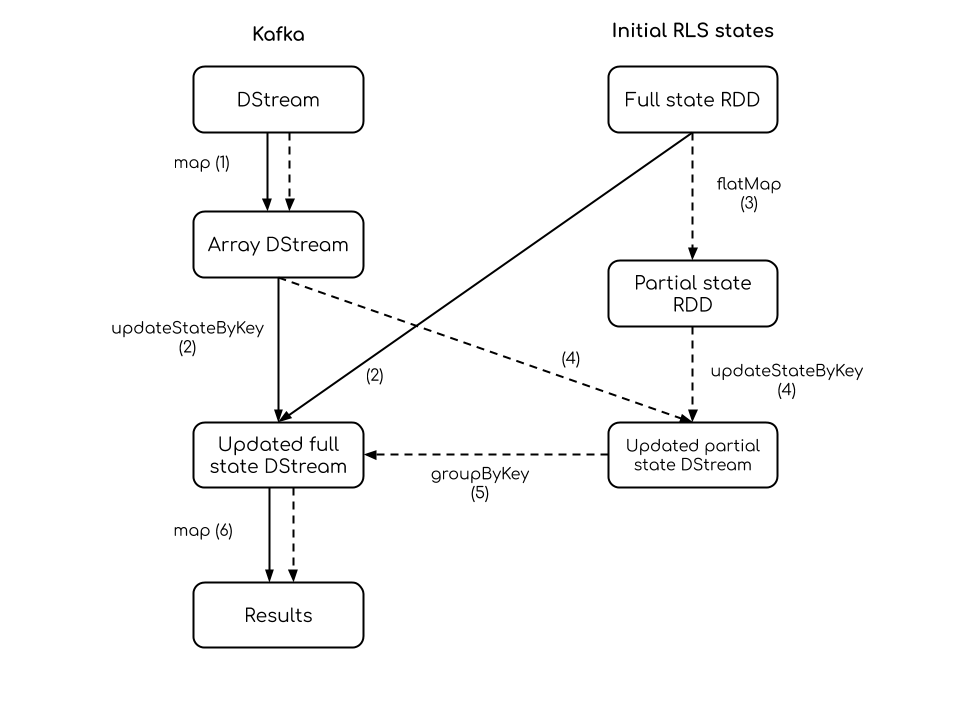
\includegraphics[width=\textwidth, keepaspectratio]{imgs/lineage-graph.png}
        \caption{Lineage graph for the proposed architecture. Dashed lines indicate
            the Spark transformations applied in the distributed version
            and plain lines indicate the transformations applied in the fully-vectorized version.}
        \label{architecture}
    \end{center}
\end{figure}

